\documentclass[conference]{IEEEtran}
\usepackage{cite}
\usepackage{amsmath,amssymb,amsfonts}
\usepackage{algorithmic}
\usepackage{graphicx}
\usepackage{textcomp}
\usepackage{xcolor}
\graphicspath{{../Poster/}{../poster/}{../experiments/plots/}}
\def\BibTeX{{\rm B\kern-.05em{\sc i\kern-.025em b}\kern-.08em
    T\kern-.1667em\lower.7ex\hbox{E}\kern-.125emX}}
\begin{document}

\title{Portfolio RiskQ: Fast Tail Risk Estimation via Discretized IQAE}

\author{\IEEEauthorblockN{Emily Berlinghoff}
\IEEEauthorblockA{\textit{Western Quantum Club} \\
\textit{Western University}\\
London, Ontario, Canada \\
eberling@uwo.ca}
\and
\IEEEauthorblockN{Amir Orfali}
\IEEEauthorblockA{\textit{Western Quantum Club} \\
\textit{Western University}\\
London, Ontario, Canada \\
aorfali2@uwo.ca}
}

\maketitle

\begin{abstract}
Risk teams need reliable VaR/CVaR under tight compute budgets, especially when tail behavior drives capital decisions. We present a classical-to-quantum pipeline that preserves the same loss distribution, tail threshold $\ell$, and histogram while enabling IQAE-based tail probability estimation. The goal is a faster tail estimate with clear, auditable outputs that remain interpretable to stakeholders. Our workflow keeps the classical baseline in place while adding a quantum estimator side-by-side, so performance can be compared. This keeps results practical for risk review.
\end{abstract}

\begin{IEEEkeywords}
VaR, CVaR, tail risk, IQAE, nested Monte Carlo
\end{IEEEkeywords}

\section{Introduction}
Risk teams need reliable VaR/CVaR under tight compute budgets, especially when tail behavior drives capital decisions. We present a classical-to-quantum pipeline that preserves the same loss distribution, tail threshold $\ell$, and histogram while enabling IQAE-based tail probability estimation. The goal is a faster tail estimate with clear, auditable outputs that remain interpretable to stakeholders. Our workflow keeps the classical baseline in place while adding a quantum estimator side-by-side, so performance can be compared. This keeps results practical for risk review.

\section{Motivation and Project Direction}
We investigate how quantum algorithms can integrate with established financial risk workflows. The project focuses on VaR/CVaR as a cornerstone of quantitative finance, builds and validates the algorithm classically, and then evaluates a quantum simulation path to assess potential speedup.

\section{Background and Definitions}
We use the following terms throughout: VaR is a loss cutoff at confidence level $\alpha$; CVaR is the average loss beyond VaR; IQAE denotes Iterative Quantum Amplitude Estimation; and discretization refers to mapping losses into $2^n$ histogram bins. Portfolio loss is $L = -w^\top r$ with tail probability $p = \mathbb{P}(L \ge \ell)$, where the tail threshold $\ell$ defines extreme-loss events and discretization groups losses into $2^n$ bins to form a histogram.

\section{Related Work}
Classical risk measurement and Monte Carlo foundations follow standard treatments of VaR/CVaR and simulation-based estimation. Quantum amplitude estimation and its iterative variants motivate the IQAE component, and prior quantum finance work applies related methods to risk analysis under NISQ constraints. Our contribution focuses on a consistent, auditable classical-to-quantum pipeline that preserves loss distributions and tail thresholds for fair comparison. This bridges research-grade quantum estimation with production-style risk reporting, including confidence intervals and error metrics.

\section{Objectives}
\begin{itemize}
    \item Build a working classical risk engine and dashboard MVP.
    \item Add discretization and tail-mask generation.
    \item Deliver a small-scale IQAE simulator with resource reporting.
    \item Communicate results through stakeholder-friendly visuals.
\end{itemize}
The emphasis is on a pipeline that supports both classical validation and quantum-oriented estimation.

\section{Models and Materials}
Implementation uses Python with NumPy and Pandas for numerical work, a FastAPI backend for serving risk metrics, and a Streamlit + Plotly front end for interactive visualization. The model uses Gaussian returns with an optional crash-mixture scenario, nested Monte Carlo for regime uncertainty, histogram-based discretization for quantum mapping, and a backend toggle for classical versus quantum comparison.

\section{Methodology}
\subsection{Nested Monte Carlo (loss samples)}
Outer loop samples market regime parameters (e.g., drift/vol/correlation), and the inner loop draws returns from a Gaussian model to compute portfolio loss. $r$ are simulated asset returns, $\mu$ and $\Sigma$ are their mean and covariance, and $w$ are portfolio weights.
\begin{align*}
(\mu_s,\Sigma_s) \sim \mathcal{S}, \quad r_{s,i} \sim \mathcal{N}(\mu_s,\Sigma_s), \quad L_{s,i} = -w^\top r_{s,i}
\end{align*}

\subsection{Tail metrics}
VaR is the loss quantile at level $\alpha$; CVaR averages losses beyond VaR.
\begin{align*}
    \text{VaR}_{\alpha} &= Q_{\alpha}(L) \\
    \text{CVaR}_{\alpha} &= \mathbb{E}[L \mid L \ge \text{VaR}_{\alpha}]
\end{align*}

\subsection{Discretization}
\begin{itemize}
    \item Bin losses into $2^n$ intervals.
    \item Produce edges, probabilities, tail mask.
    \item Bootstrap error estimate for bin stability.
    \item Bin counts $n_i$ define histogram probabilities $p_i$; tail probability is the sum over tail bins.
\end{itemize}
\begin{align*}
    p_i &= \frac{n_i}{N}, \quad \sum_i p_i = 1, \quad \hat{p} = \sum_{i \in \text{tail}} p_i
\end{align*}

\subsection{IQAE (simulator)}
\begin{itemize}
    \item Uses Grover iteration schedule to amplify tail states.
    \item Returns estimate with confidence interval.
    \item IQAE probes multiple Grover powers $m$ to infer $p$ from amplified measurements.
\end{itemize}
\begin{align*}
    p &= \sin^2(\theta), \quad p_m = \sin^2((2m+1)\theta)
\end{align*}

\section{Experimental Setup}
Experiments vary the number of Monte Carlo paths, the number of IQAE oracle calls, the discretization resolution ($2^n$ bins), and the noise level in the simulator. The return model is Gaussian with an optional crash-mixture scenario, and regime uncertainty is handled with nested Monte Carlo. Histogram-based discretization supports quantum mapping, and a backend toggle compares classical and quantum paths. Results compare classical and quantum estimates using the same threshold $\ell$ and histogram.

\section{Evaluation Metrics}
We report absolute tail-probability error against a known baseline and track IQAE confidence intervals. The classical curve provides a sanity check on $1/\sqrt{N}$ behavior, while the IQAE curve shows how a few Grover rounds can capture most of the tail probability. Discretization and noise sweeps show the practical regime where IQAE comparisons remain stable. Resource usage (qubits, depth, 2Q gates, oracle calls) is recorded to characterize feasibility.

\section{System Pipeline (Classical to Quantum)}
Market data calibrates $(\mu,\sigma)$, nested MC yields losses, and discretization builds a $2^n$ histogram and tail mask in the classical pipeline. IQAE then estimates tail probability in the quantum stage.

\section{Analysis and Results}
We validated probability normalization and tail-mask correctness, compared IQAE estimates to true tail probability on toy data, and tracked resource usage (qubits, depth, 2Q gates, oracle calls). Classical and quantum estimates used the same $\ell$ and histogram, and the dashboard reported VaR/CVaR with a tail-highlighted histogram.

\section{Key Contribution}
We present a classical-to-quantum VaR/CVaR workflow that uses a discretized histogram and tail mask to enable IQAE comparison against nested Monte Carlo. We also map feasibility boundaries for NISQ constraints and validate the pipeline in a production-style dashboard. This bridges research-grade quantum estimation with production-style risk reporting, including confidence intervals and error metrics.

\section{Experiment Visuals}
These plots summarize accuracy tradeoffs across classical sampling, quantum query cost, discretization resolution, and noise sensitivity, as shown in Fig.~\ref{fig:exp-classical-quantum} and Fig.~\ref{fig:exp-discretization-noise}. We report absolute tail-probability error against a known baseline, highlighting where additional compute yields diminishing returns and where noise dominates estimation error. The classical curve provides a sanity check on $1/\sqrt{N}$ behavior, while the IQAE curve shows how a few Grover rounds can capture most of the tail probability. Discretization and noise sweeps show the practical regime where IQAE comparisons remain stable.

\begin{figure}[!t]
    \centering
    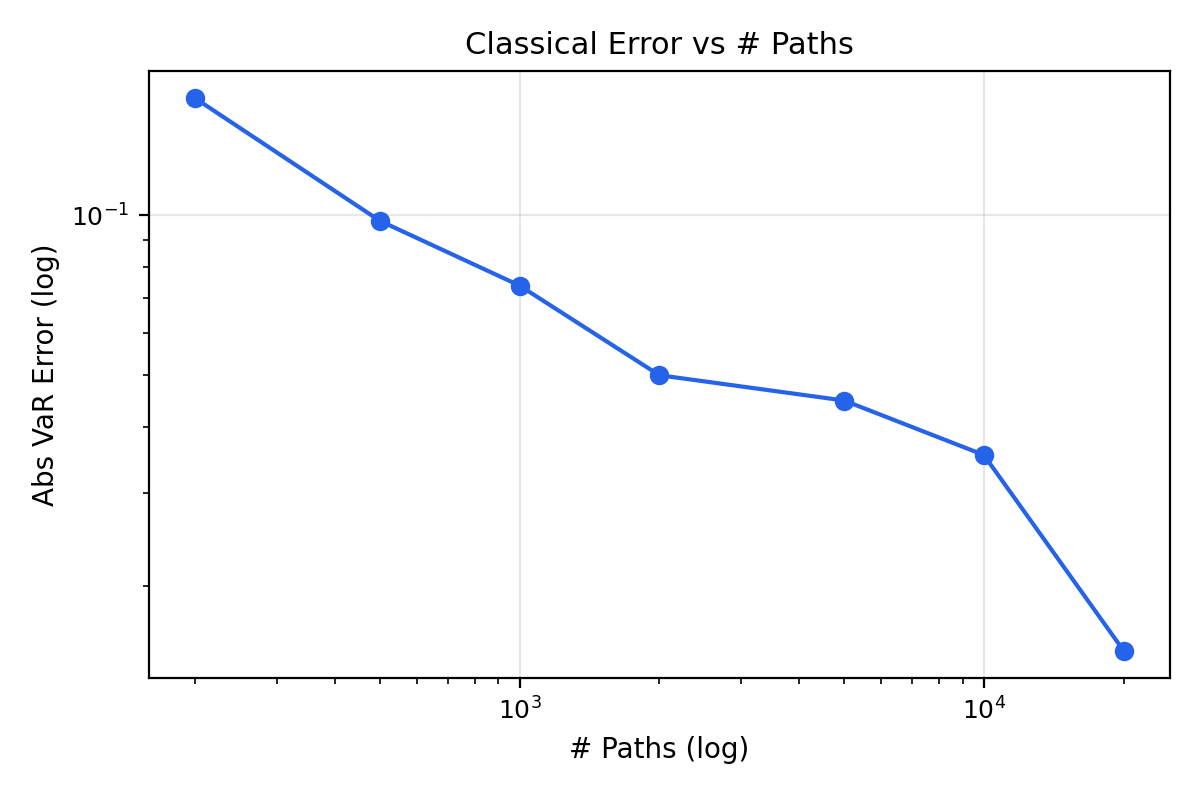
\includegraphics[width=0.48\linewidth]{classical_error_vs_paths.png}\hfill
    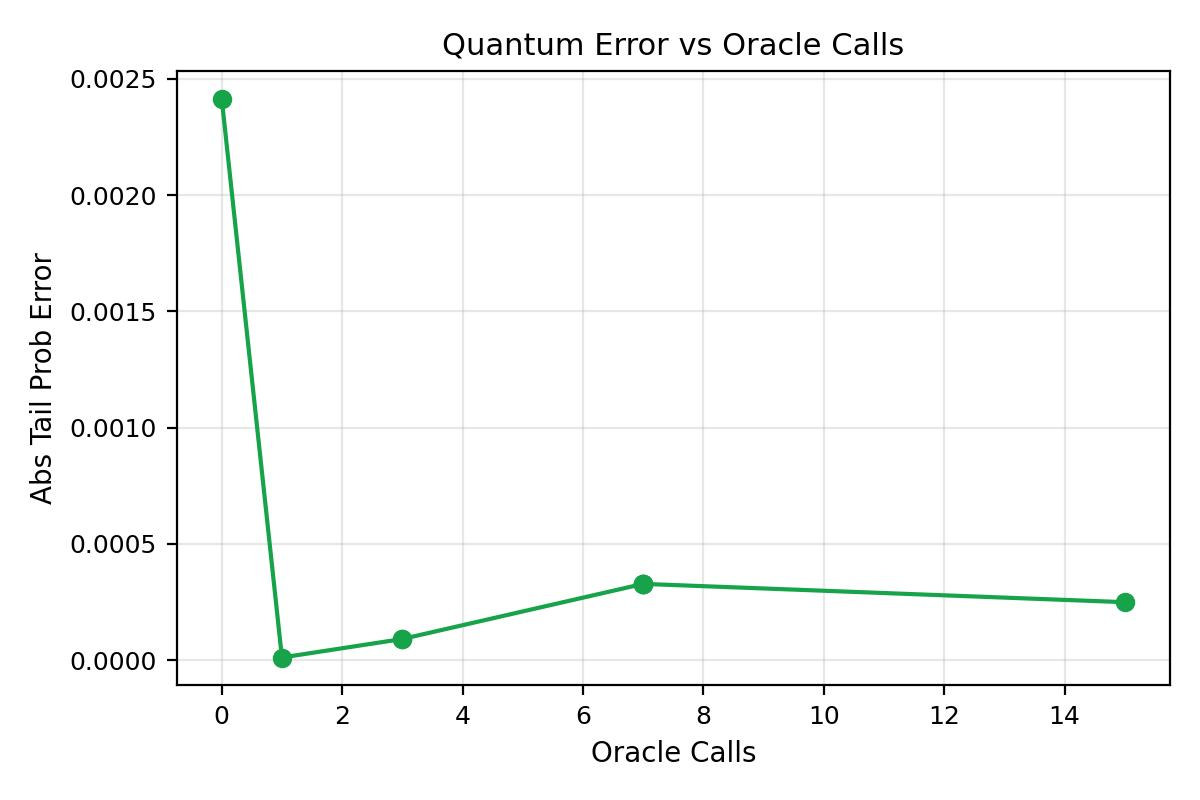
\includegraphics[width=0.48\linewidth]{quantum_error_vs_oracle_calls.png}
    \caption{Classical Error vs MC Paths (left) and Quantum Error vs Oracle Calls (right).}
    \label{fig:exp-classical-quantum}
\end{figure}

\begin{figure}[!t]
    \centering
    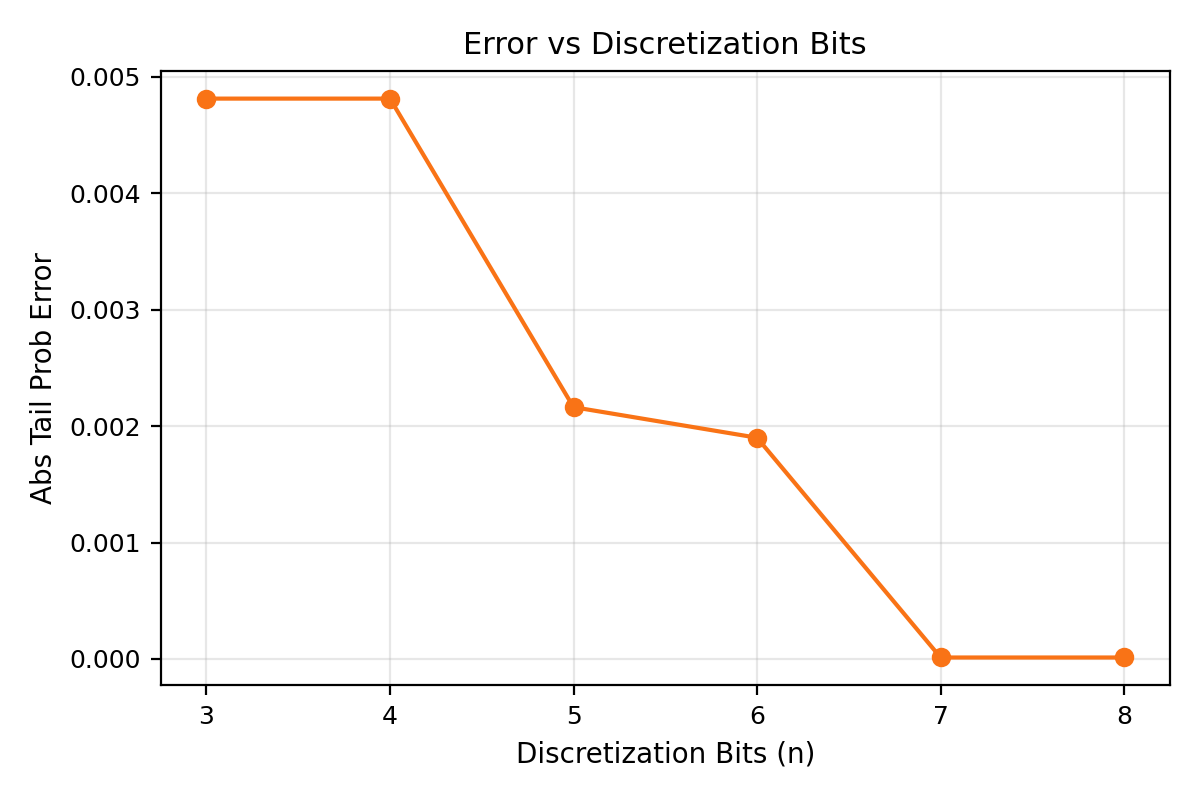
\includegraphics[width=0.48\linewidth]{error_vs_discretization_bits.png}\hfill
    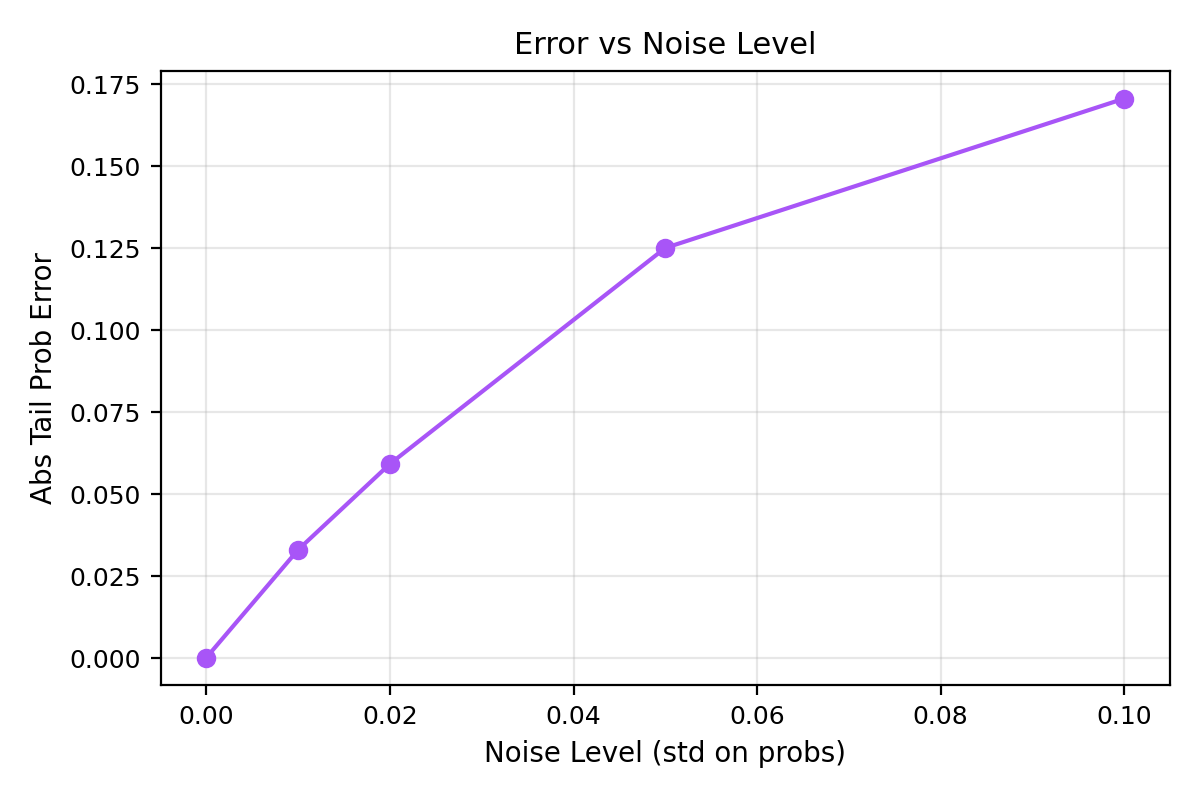
\includegraphics[width=0.48\linewidth]{error_vs_noise_level.png}
    \caption{Error vs Discretization Bits (left) and Error vs Noise Level (right).}
    \label{fig:exp-discretization-noise}
\end{figure}

\section{Feasibility Boundary}
In the feasible region, resource demands stay low enough for near-term devices, while the borderline region signals settings that quickly become impractical. The not-viable region reflects NISQ-era limits where IQAE cost dominates the workflow (Fig.~\ref{fig:feasibility-boundary}). Bands use a composite resource score (qubits + depth + oracle calls).
\begin{figure}[!t]
    \centering
    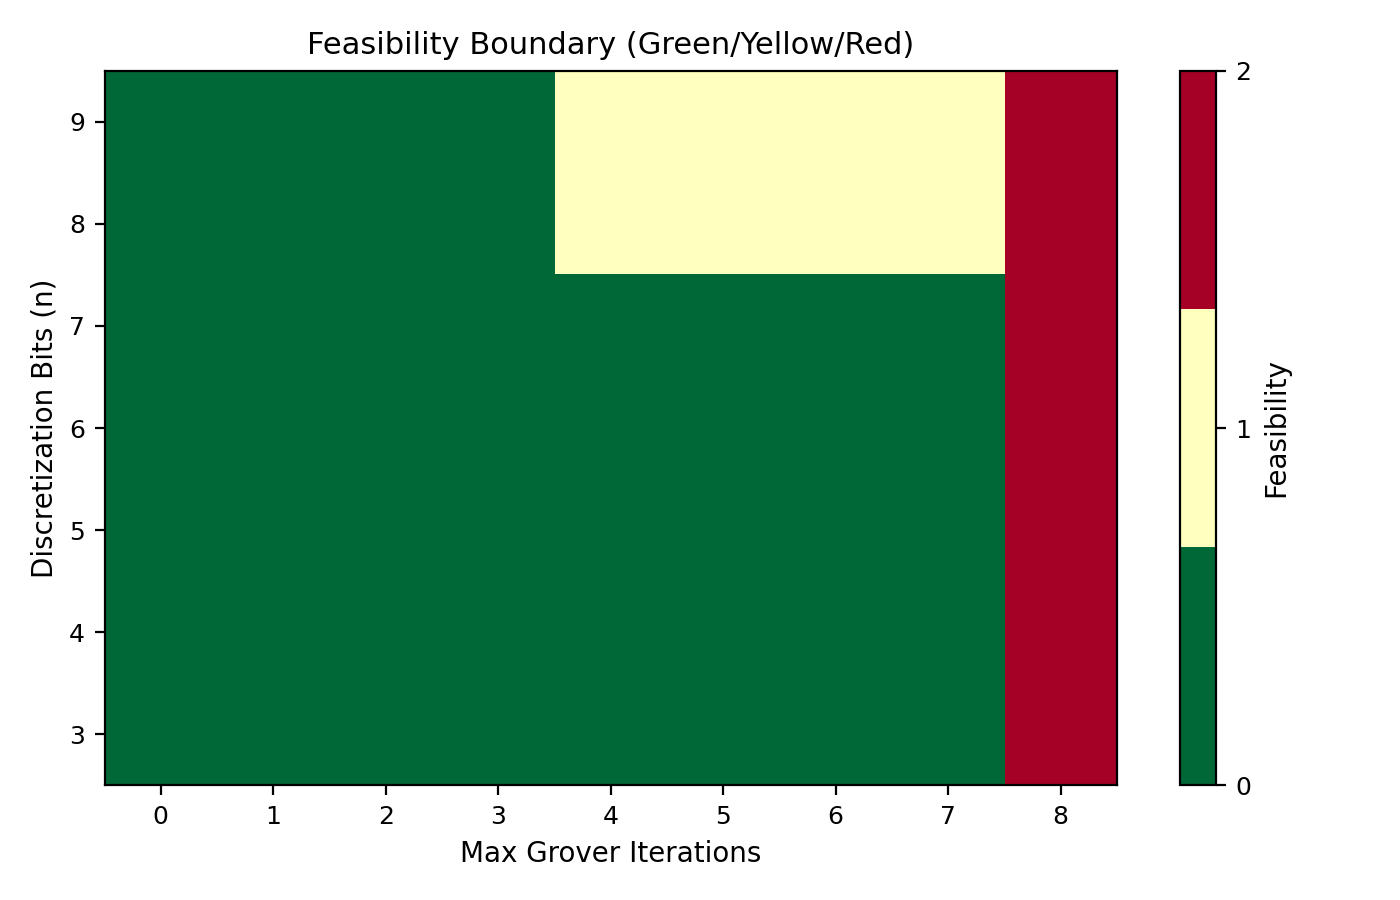
\includegraphics[width=0.7\linewidth]{feasibility_boundary.png}
    \caption{Feasibility boundary based on composite resource score.}
    \label{fig:feasibility-boundary}
\end{figure}

\section{Dashboard Visuals}
Left panel collects portfolio inputs and stress settings; right panel reports VaR/CVaR, a tail-highlighted histogram, and a classical vs quantum comparison (Fig.~\ref{fig:dashboard}). IQAE reports the same tail probability with a confidence interval and absolute/relative error.
\begin{figure}[!t]
    \centering
    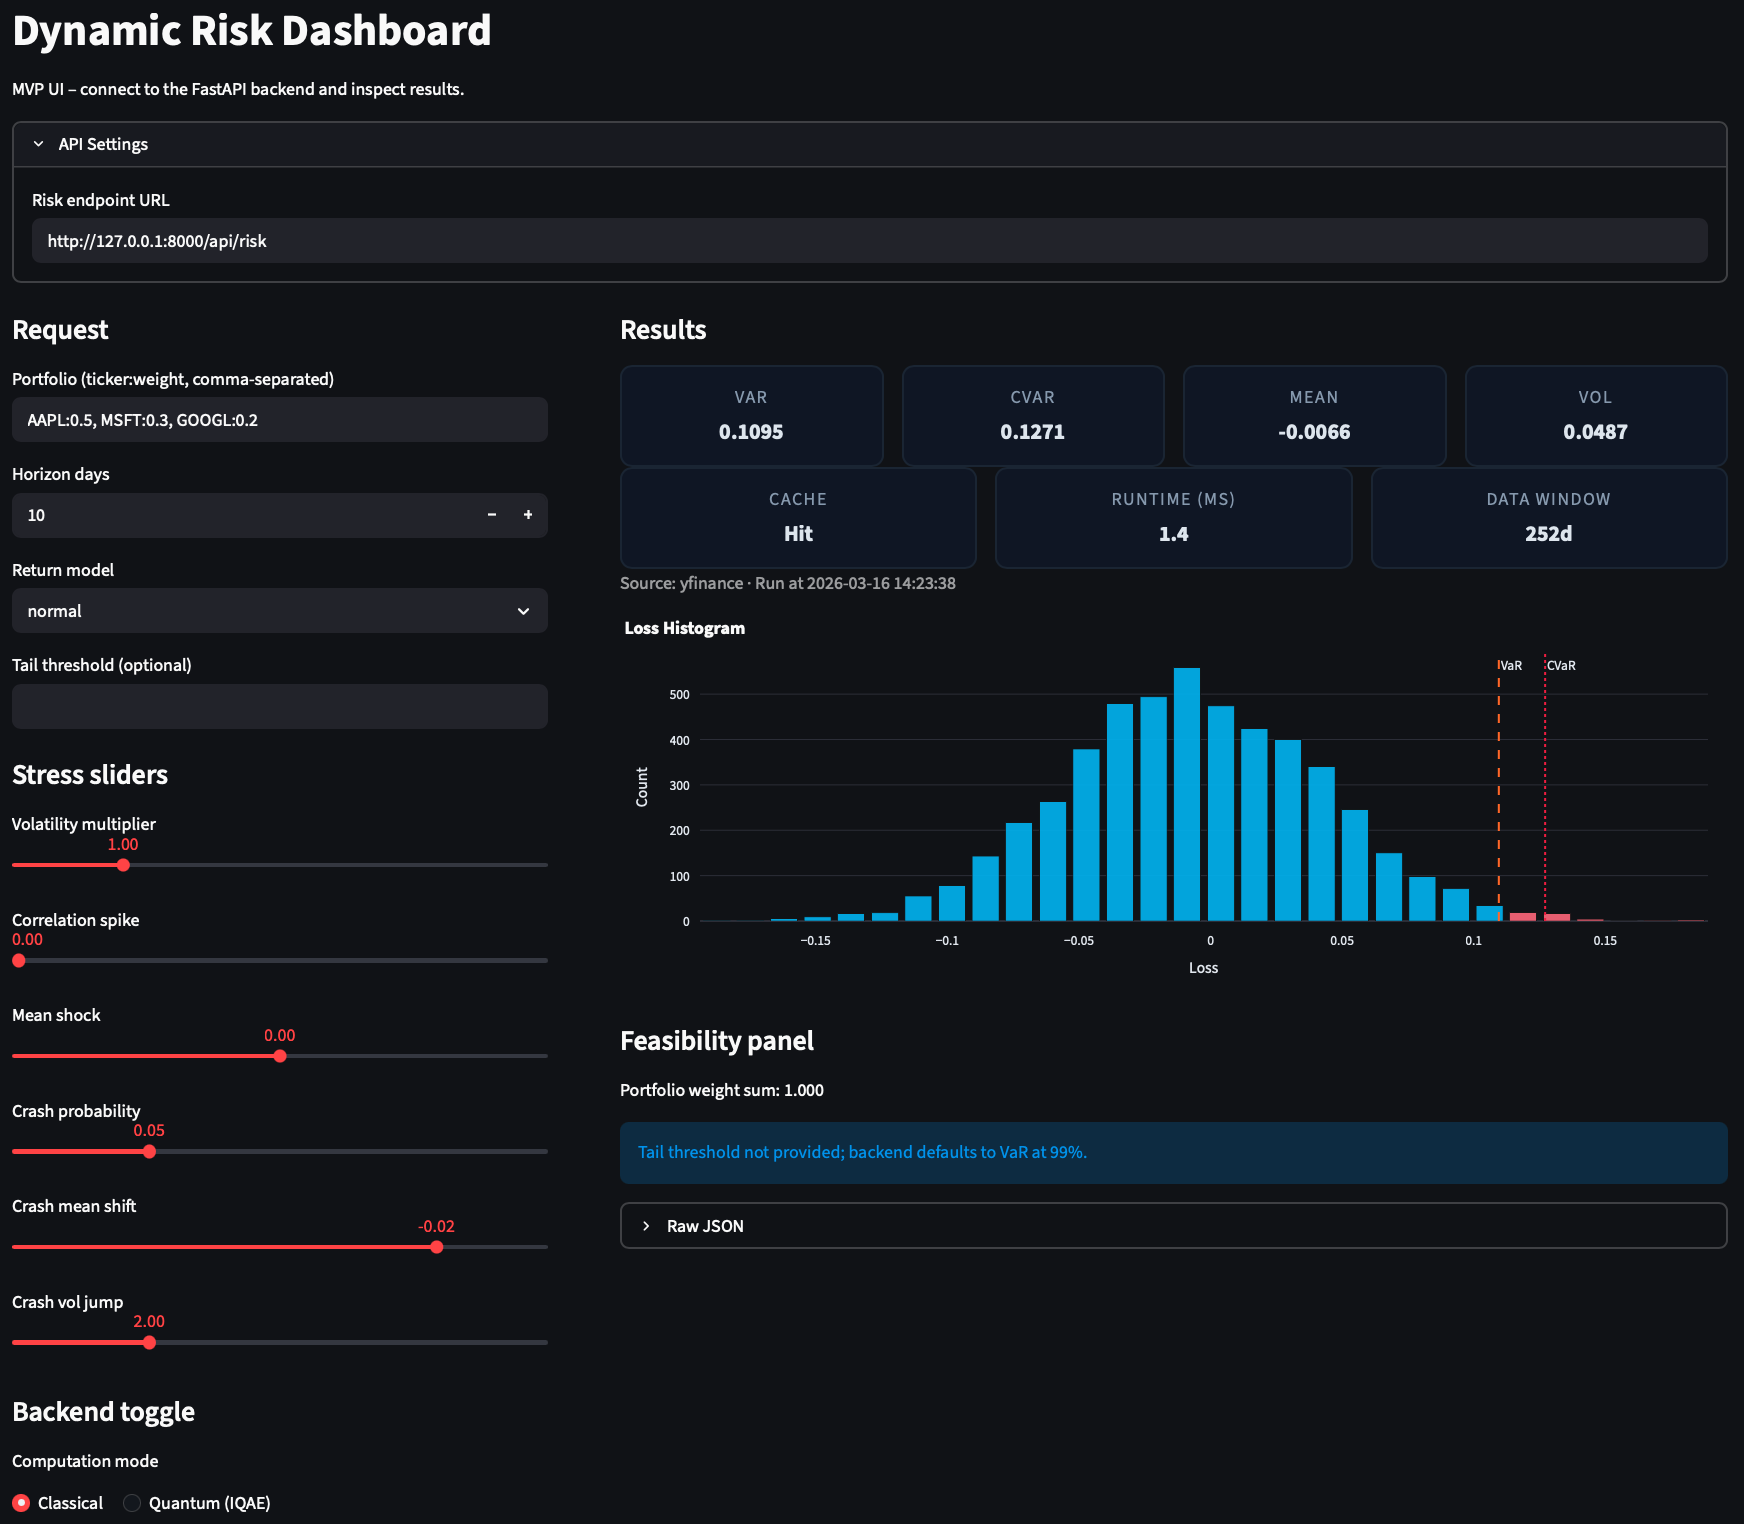
\includegraphics[width=0.48\linewidth]{c_dash.png}\hfill
    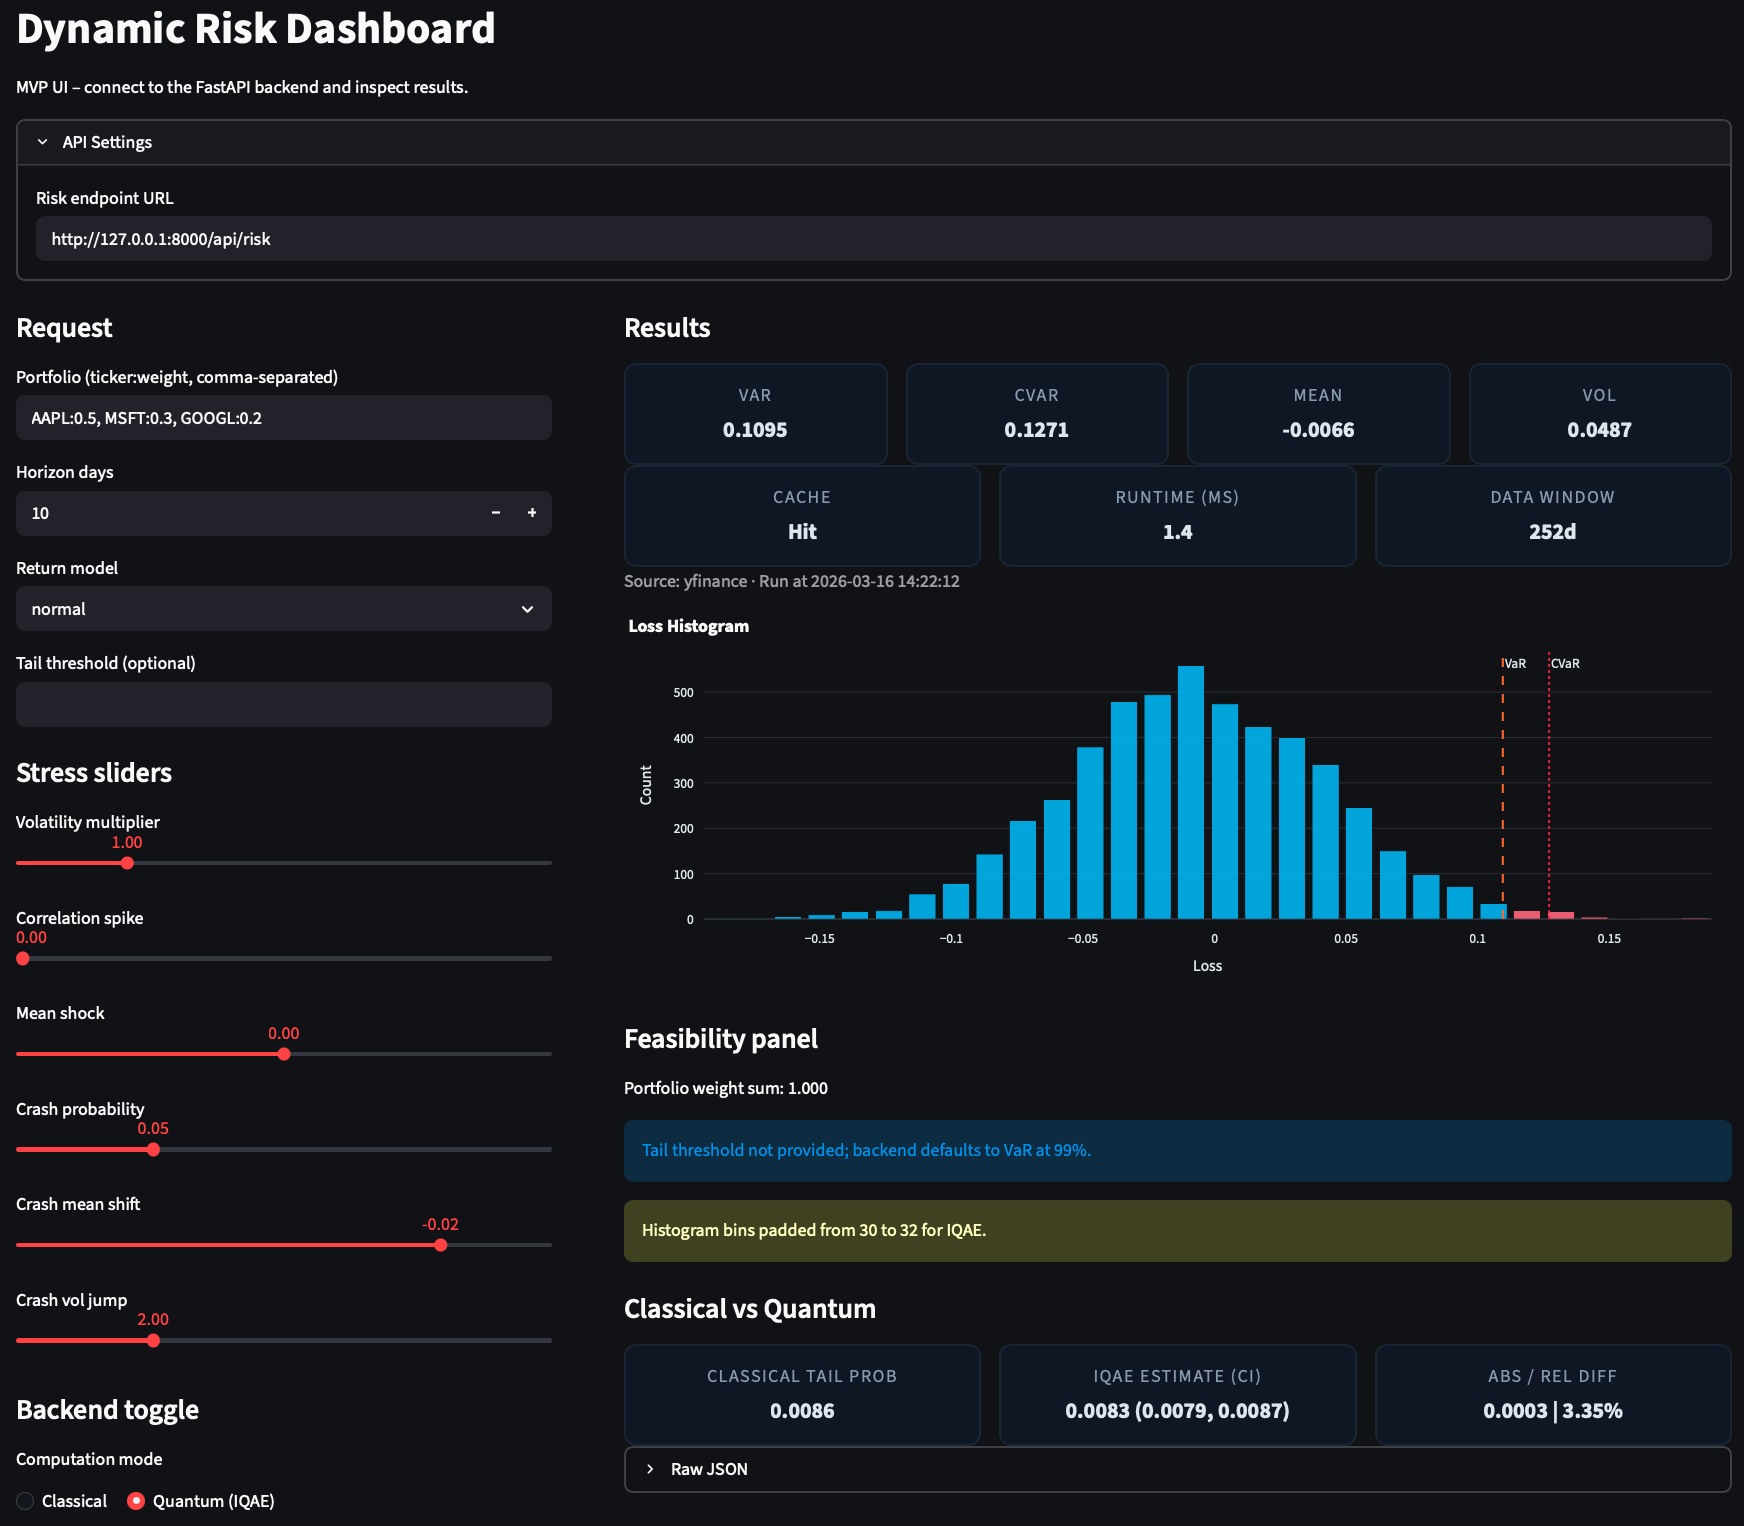
\includegraphics[width=0.48\linewidth]{q_dash.png}
    \caption{Classical Backend (left) and Quantum (IQAE) Backend (right).}
    \label{fig:dashboard}
\end{figure}

\section{Discussion and Implications}
Discretization provides a stable bridge to IQAE, simulator estimates align with expected tail probabilities, and resource reports clarify near-term feasibility limits. Comparisons use the same threshold $\ell$, scenario, and histogram, and IQAE estimates match classical tail probability on toy data.

\section{Who Is Pursuing This Currently?}
\subsection{Industry Activity}
J.P. Morgan Chase, Goldman Sachs, HSBC, Barclays, and BNP Paribas are active in quantum finance initiatives. Reported efforts include in-house algorithm development for pricing and risk, JPMorgan demonstrations of quantum algorithms on hardware (Barron), and IBM--JPMorgan collaborations on portfolio optimization and derivatives pricing.

\section{Limitations}
Results are based on simulator studies and toy data, and feasibility conclusions reflect NISQ-era resource constraints. The evaluation emphasizes comparability and auditability rather than end-to-end performance on production-scale portfolios, and settings in the not-viable region reflect NISQ-era limits where IQAE cost dominates the workflow.

\section{Reproducibility}
Code and dashboard materials are available at the project repository listed in the Acknowledgment section.

\section{Conclusion}
The MVP validates a classical-to-quantum risk pipeline with consistent inputs, interpretable outputs, and a clear audit trail from data to tail estimate. IQAE offers a potential quadratic reduction in sampling complexity; our results focus on comparability and feasibility under near-term constraints.

\section*{Acknowledgment}
Western Quantum Club \& Western University.\\
\texttt{aorfali2@uwo.ca \quad eberling@uwo.ca}\\
\texttt{https://github.com/amirorfali/Dynamic-Risk-Dashboard}

\begin{thebibliography}{00}
\bibitem{ref1} Rockafellar \& Uryasev (2000) CVaR, \emph{Journal of Risk}.
\bibitem{ref2} Jorion (2007) \emph{Value at Risk}.
\bibitem{ref3} Glasserman (2004) \emph{Monte Carlo Methods in Financial Engineering}.
\bibitem{ref4} Brassard et al. (2002) QAE, \emph{Contemporary Mathematics}.
\bibitem{ref5} Grinko et al. (2021) Iterative QAE, \emph{npj Quantum Information}.
\bibitem{ref6} Grover (1996) STOC.
\bibitem{ref7} Woerner \& Egger (2019) quantum risk analysis, \emph{npj Quantum Information}.
\bibitem{ref8} Amiet \& Wehner (2020) NISQ finance algorithms, \emph{npj Quantum Information}.
\end{thebibliography}

\end{document}
